\begin{frame}
\frametitle{Quantum theory of radiation by nonstationary systems
        with application to high-order harmonic generation
        (Phys. Rev. A 101, 013410 (2020))}
        \framesubtitle{Transition amplitudes - gauge-related convergence}
\small
\begin{textblock*}{500pt}(5pt,60pt)
%\centering
%\rotatebox{90}{
 \begin{minipage}{0.0\linewidth}
 \begin{figure}[tp]
 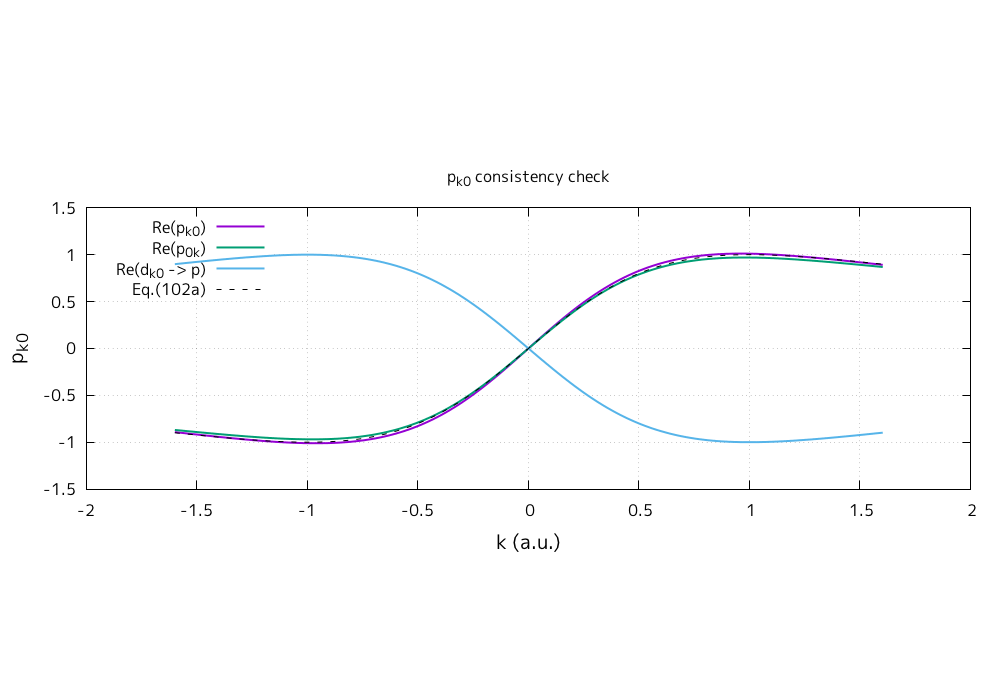
\includegraphics[scale=.18, trim={6 180 10 185},clip]{images/pk0_40_200_8000.png} \\
 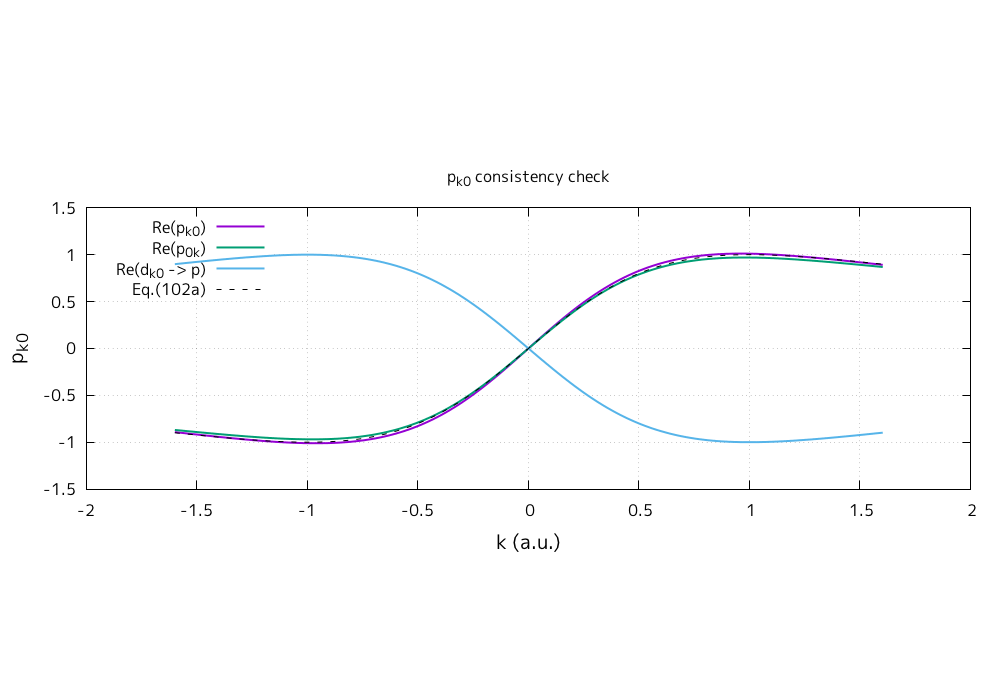
\includegraphics[scale=.18, trim={6 180 10 185},clip]{images/pk0_40_200_8000.png} \\
%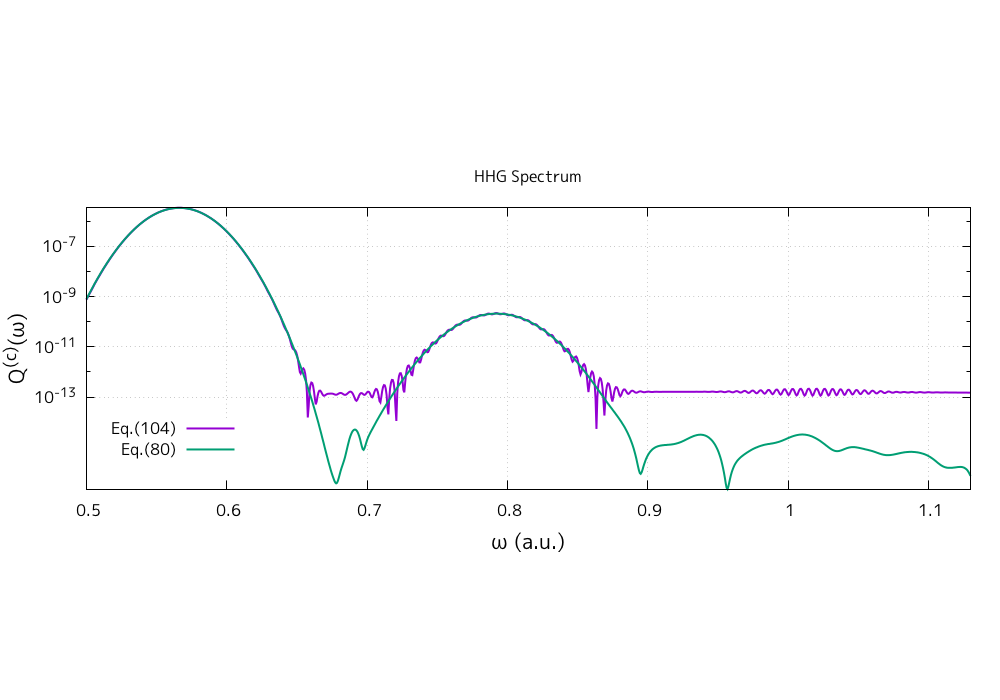
\includegraphics[scale=.18, trim={6 170 10 185},clip]{images/hhg_20_100_20000.png} 
%%\caption{Eigenvalues.}
%\label{fig:pemd_0114}
 \end{figure}

\end{minipage}
\end{textblock*}


\begin{textblock*}{500pt}(180pt,60pt)
%\centering
%\rotatebox{90}{
 \begin{minipage}{0.0\linewidth}
 \begin{figure}[tp]
 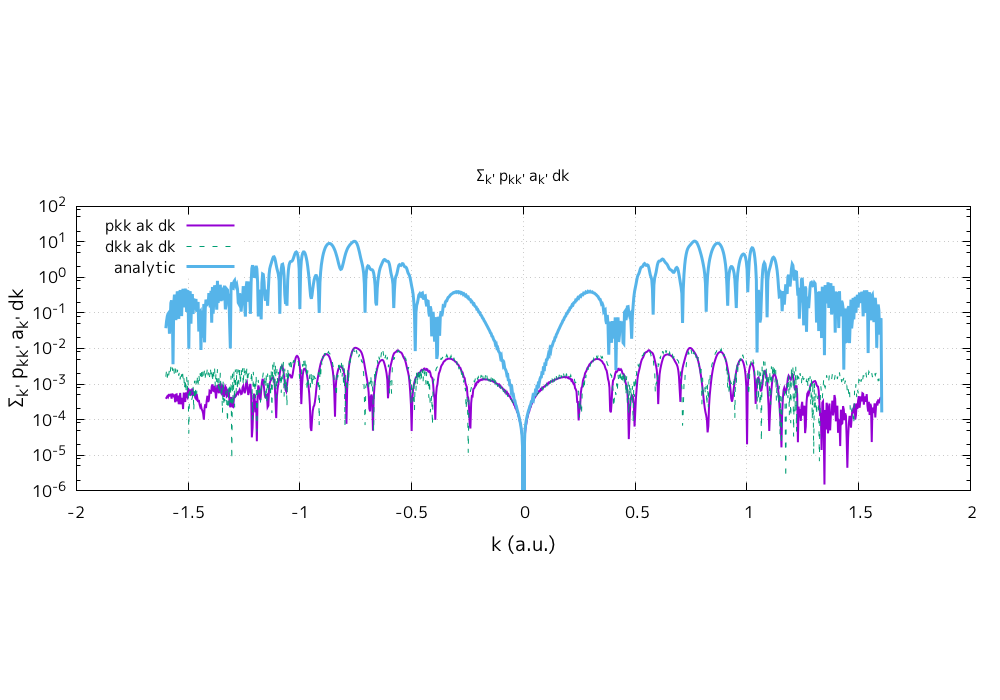
\includegraphics[scale=.18, trim={6 180 10 185},clip]{images/pkl_20_100_2000.png} \\
 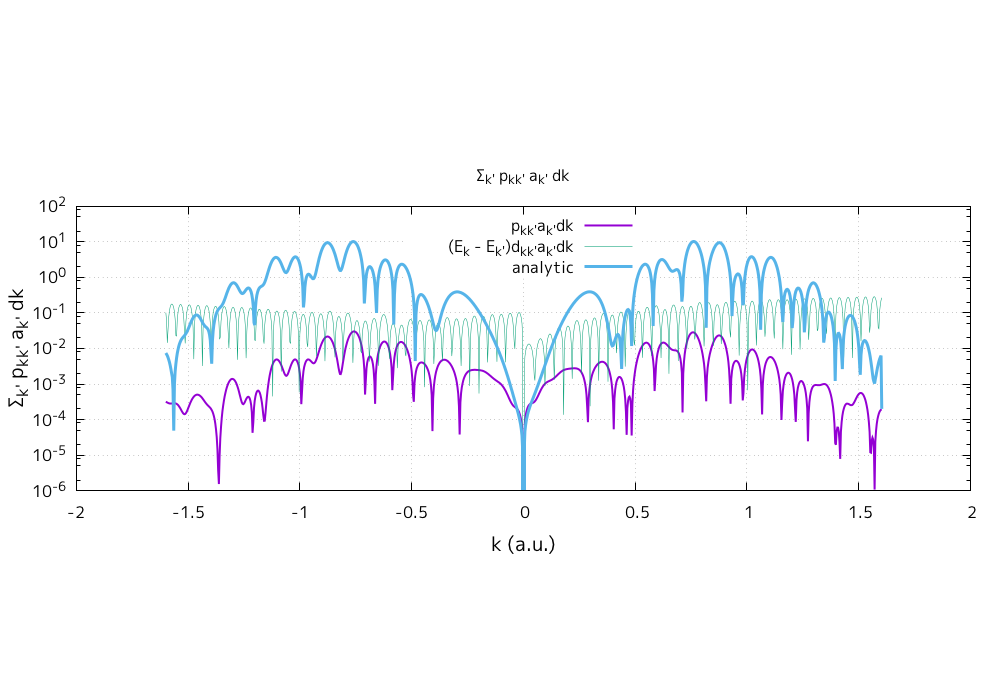
\includegraphics[scale=.18, trim={6 180 10 185},clip]{images/pkl_40_200_8000.png} \\
% 
\includegraphics[scale=.20, trim={30 130 10 130},clip]{images/114_f003_12_07_hhg.png} 

%%\caption{Eigenvalues.}
%\label{fig:pemd_0114}
 \end{figure}

\end{minipage}
\end{textblock*}


%\begin{textblock*}{500pt}(390pt,165pt)
%%\centering
%\rotatebox{90}{
% \begin{minipage}{0.0\linewidth}
% \begin{figure}[tp]
% 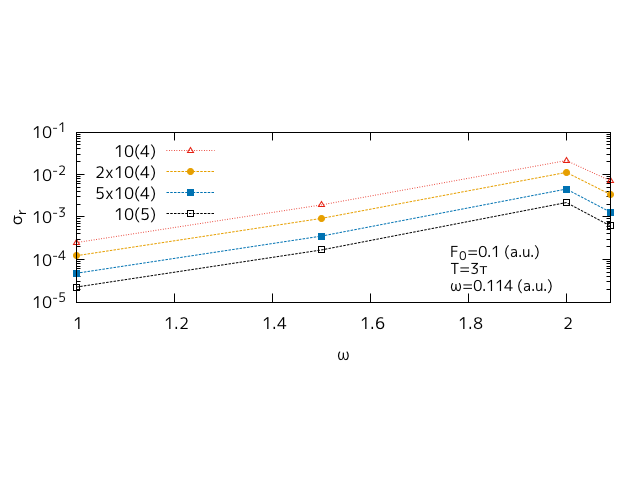
\includegraphics[scale=.20, trim={6 100 10 120},clip]{images/114_f01_3_error.png } \\
%%%\caption{Eigenvalues.}
%%\label{fig:pemd_0114}
% \end{figure}
%\end{minipage}
%}
%}
%\end{textblock*}
%
%
%
%
\begin{textblock*}{200pt}(300pt,130pt)
\rotatebox{0}{
\begin{minipage}{\linewidth}
{
\scriptsize
\centering
        \begin{align}
                \rm{Np} = 20,\;\;\;\rm{Ns} = 100 \nonumber\\
                \rm{xmax} \sim \rm{Np\,Ns} /2 \nonumber\\
                \omega_0 = 0.114\,{\rm a.u}\nonumber\\
                F_0 = 0.03\,{\rm a.u}, \;\;T=8\tau\nonumber
        \end{align}
%       \textcolor{red}{\textbf{The nonconvergence come from the fact that}
%       $\rm{xmax}\sim \rm{Np\,Ns}$ here}

}
\end{minipage}
}
\end{textblock*}


\begin{textblock*}{150pt}(20pt,230pt)
\rotatebox{0}{
\begin{minipage}{\linewidth}
{
\scriptsize
\centering
        U:  $\rm {Np}=20, \rm{Ns}=100,\; \rm{xmax}=1000$\\
        D:  $\rm {Np}=40, \rm{Ns}=200,\; \rm{xmax}=4000$\\
}
\end{minipage}
}
\end{textblock*}


\begin{textblock*}{\linewidth}(20pt,170pt)
\rotatebox{0}{
\begin{minipage}{\linewidth}
{
%\input{tables/114_f01_3t_error_2.tab}
}
\end{minipage}
}
\end{textblock*}


\begin{textblock*}{220pt}(200pt,200pt)
\scriptsize
%
\begin{align}
p_{k0} & = \int dx\,\psi_k^{(-)*}(x)\,\hat{p}\, \psi_0(x) \label{eqn:eq_pk0}\\
	\sum_{k^\prime} \Big| p_{kk^\prime}a_k \Big| dk 
      & = \sum_{k^\prime} \Big| \int dx\, \psi_k^{(-)*}(x)\,\hat{p}\,\psi_{k^\prime}^{(-)}(x) a_k \Big| dk \label{eqn:eq_pkkak}
\end{align}

\end{textblock*}

\end{frame}




%\begin{frame}
%\frametitle{Quantum theory of radiation by nonstationary systems
%        with application to high-order harmonic generation
%        (Phys. Rev. A 101, 013410 (2020))}
%        \framesubtitle{Convergence for the homogeneous problem - closure}
%\small
%\begin{textblock*}{500pt}(5pt,60pt)
%%\centering
%%\rotatebox{90}{
% \begin{minipage}{0.0\linewidth}
% \begin{figure}[tp]
% 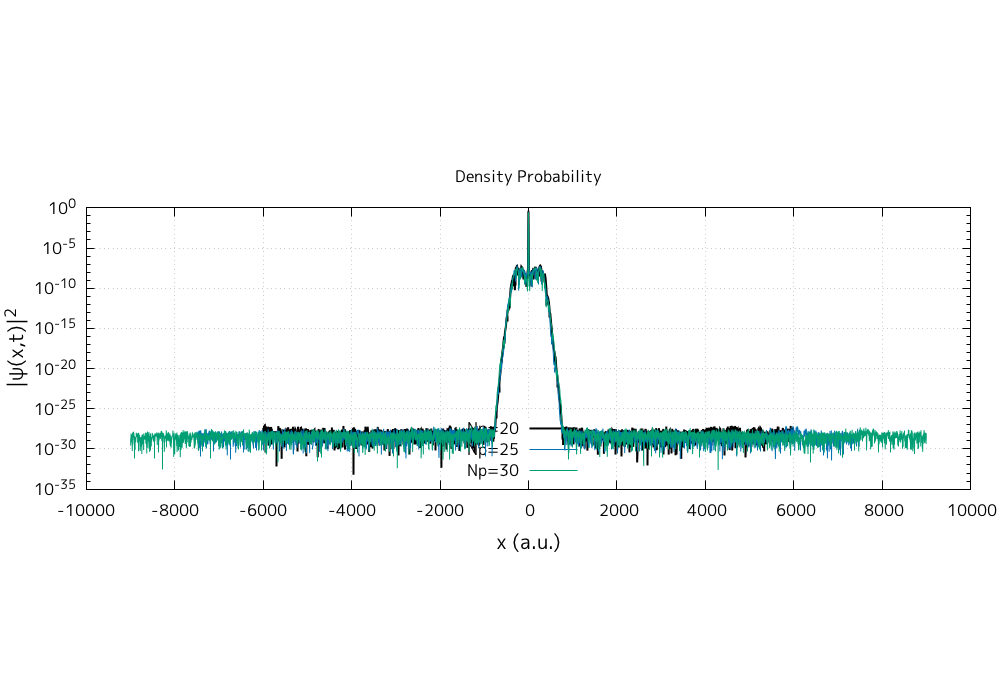
\includegraphics[scale=.18, trim={6 180 10 185},clip]{images/psi_comp_file_2npns_np20_25_30_1.png} \\
% 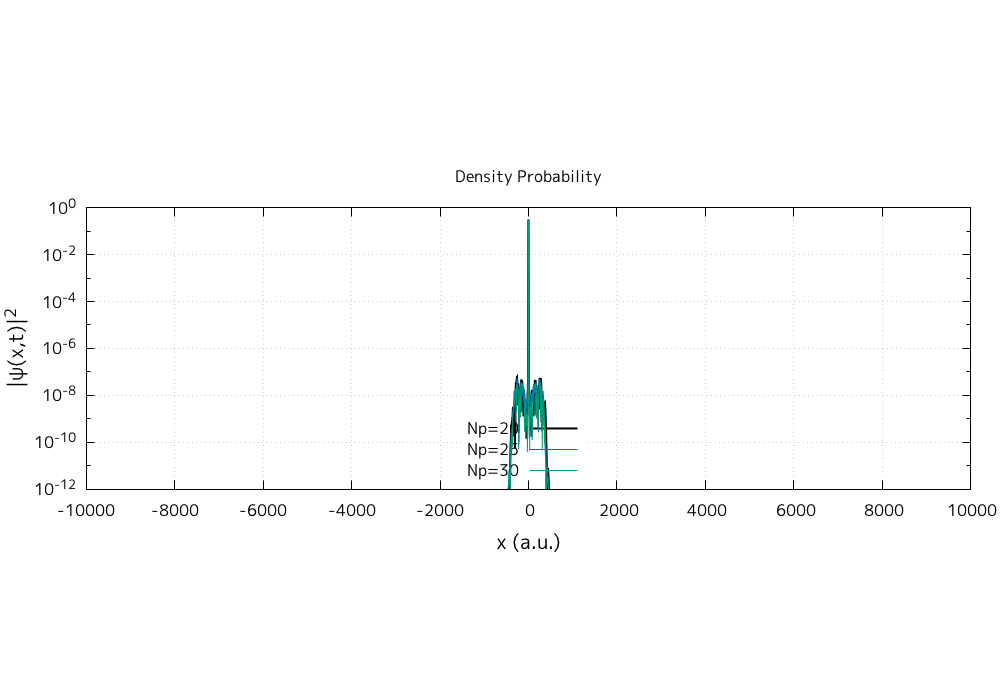
\includegraphics[scale=.18, trim={6 180 10 185},clip]{images/psi_comp_file_2npns_np20_25_30.png} \\
%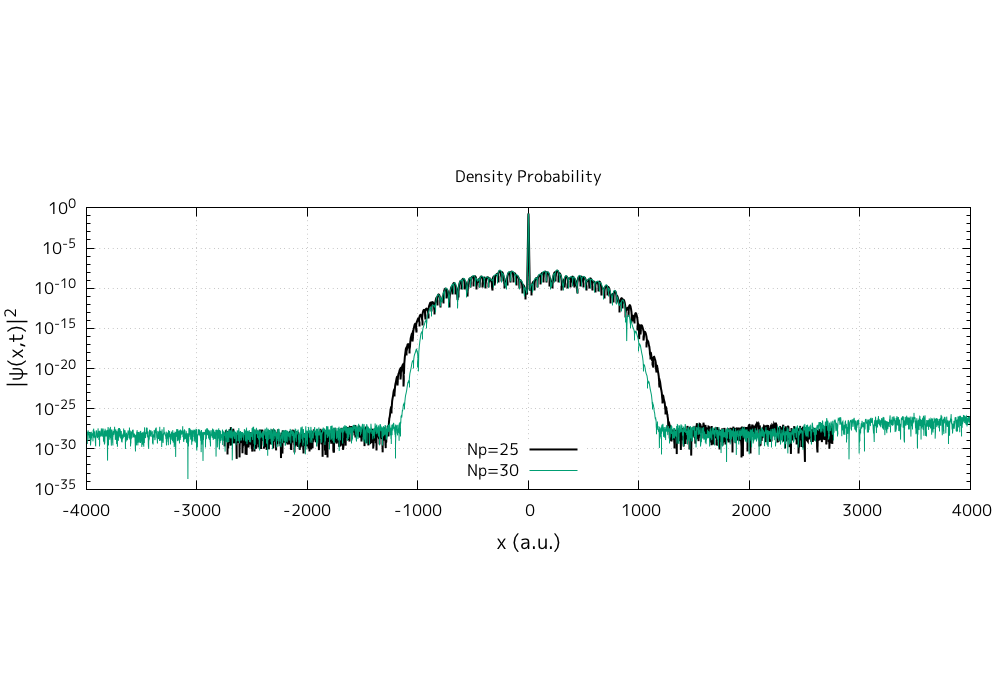
\includegraphics[scale=.18, trim={6 150 10 185},clip]{images/psi_comp_file_np25_30.png} 
%%%\caption{Eigenvalues.}
%%\label{fig:pemd_0114}
% \end{figure}
%
%\end{minipage}
%\end{textblock*}
%
%
%\begin{textblock*}{500pt}(180pt,60pt)
%%\centering
%%\rotatebox{90}{
% \begin{minipage}{0.0\linewidth}
% \begin{figure}[tp]
% 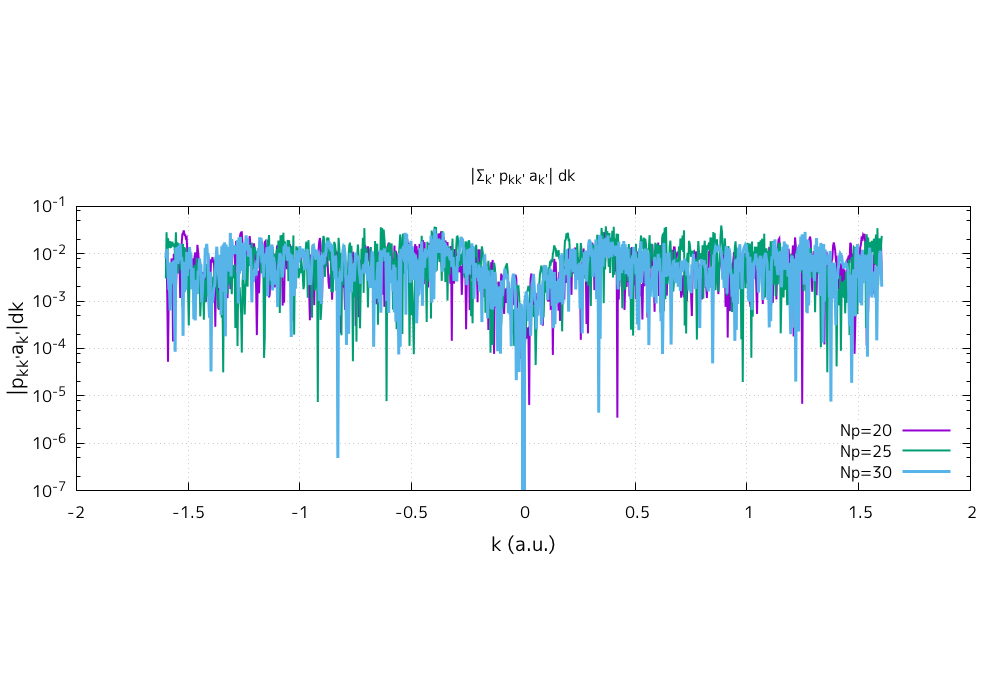
\includegraphics[scale=.18, trim={6 180 10 185},clip]{images/pkkakdk_comp_file_2npns_np20_25_30.png} \\
% 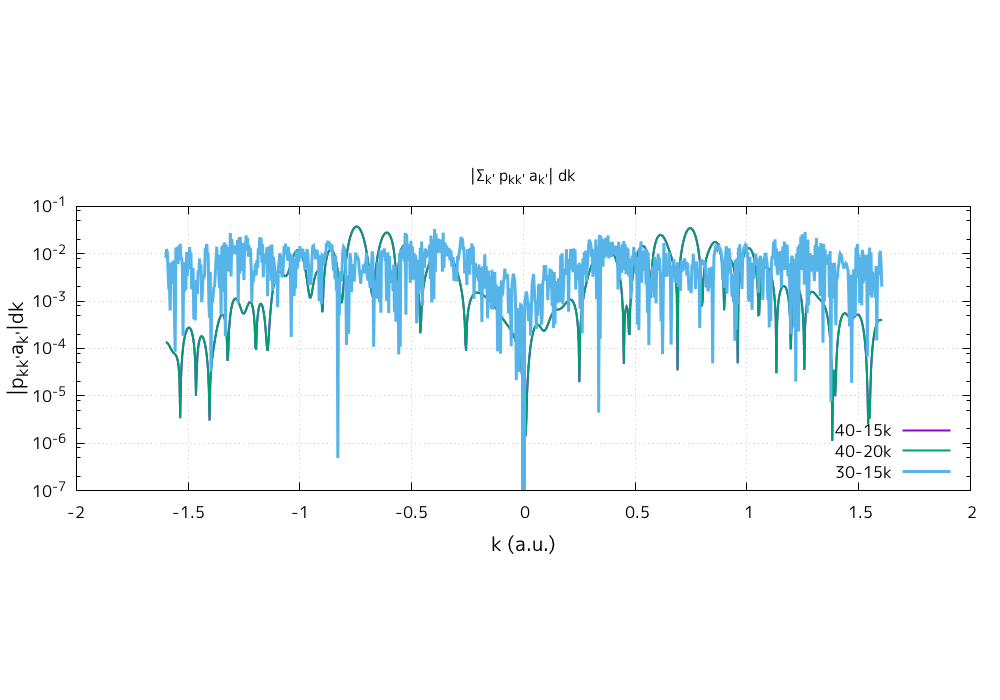
\includegraphics[scale=.18, trim={6 180 10 185},clip]{images/pkkakdk_comp_file_2npns_np40_15_20_np30_15.png} \\
%% 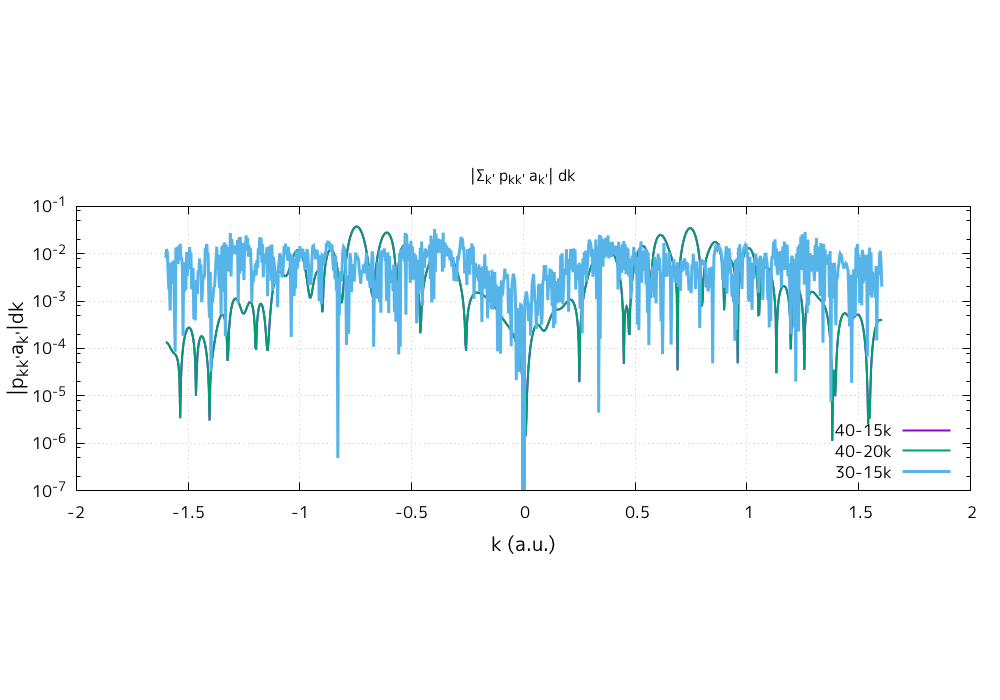
\includegraphics[scale=.18, trim={6 150 10 185},clip]{images/pkkakdk_comp_file_2npns_np40_15_20_np30_15.png} 
%
%%%\caption{Eigenvalues.}
%%\label{fig:pemd_0114}
% \end{figure}
%
%\end{minipage}
%\end{textblock*}
%
%
%%\begin{textblock*}{500pt}(390pt,165pt)
%%%\centering
%%\rotatebox{90}{
%% \begin{minipage}{0.0\linewidth}
%% \begin{figure}[tp]
%% 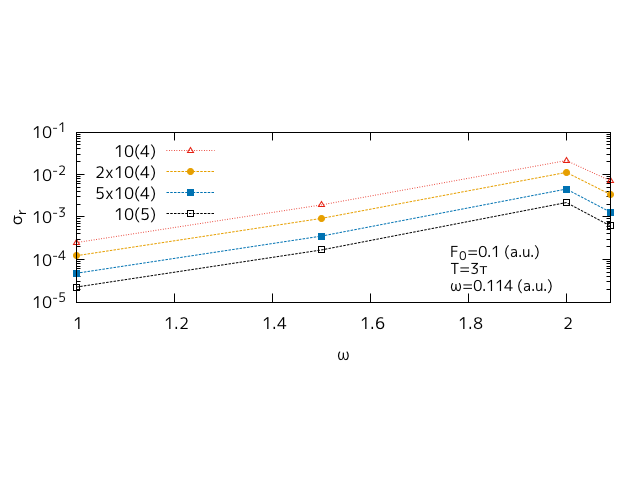
\includegraphics[scale=.20, trim={6 100 10 120},clip]{images/114_f01_3_error.png } \\
%%%%\caption{Eigenvalues.}
%%%\label{fig:pemd_0114}
%% \end{figure}
%%\end{minipage}
%%}
%%}
%%\end{textblock*}
%%
%%
%%
%%
%\begin{textblock*}{200pt}(300pt,130pt)
%\rotatebox{0}{
%\begin{minipage}{\linewidth}
%{
%\scriptsize
%\centering
%        \begin{align}
%%               \rm{Np} = x0,\;\;\;\rm{Ns} = 200 \nonumber\\
%                \:\:\;\;\;\rm{Ns} = 200 \nonumber\\
%                \rm{xmax} \sim \rm{Np\,Ns} \nonumber\\
%                \omega_0 = 0.114\,{\rm a.u}\nonumber\\
%                F_0 = 0.03\,{\rm a.u}, \;\;T=5\tau\nonumber
%        \end{align}
%%       \textcolor{red}{\textbf{The nonconvergence come from the fact that}
%%       $\rm{xmax}\sim \rm{Np\,Ns}$ here}
%
%}
%\end{minipage}
%}
%\end{textblock*}
%
%
%%\begin{textblock*}{150pt}(20pt,230pt)
%%\rotatebox{0}{
%%\begin{minipage}{\linewidth}
%%{
%%\scriptsize
%%\centering
%%        U:  $\rm {Np}=20, \rm{Ns}=100,\; \rm{xmax}=1000$\\
%%        D:  $\rm {Np}=40, \rm{Ns}=200,\; \rm{xmax}=4000$\\
%%}
%%\end{minipage}
%%}
%%\end{textblock*}
%
%
%\begin{textblock*}{\linewidth}(20pt,170pt)
%\rotatebox{0}{
%\begin{minipage}{\linewidth}
%{
%%\input{tables/114_f01_3t_error_2.tab}
%}
%\end{minipage}
%}
%\end{textblock*}
%
%
%
%\begin{textblock*}{220pt}(200pt,200pt)
%\scriptsize
%%
%\begin{align}
%p_{k0} & = \int dx\,\psi_k^{(-)*}(x)\,\hat{p}\, \psi_0(x) \tag{\ref{eqn:eq_pk0}}
% \\
%	\sum_{k^\prime} \Big| p_{kk^\prime}a_k \Big| dk 
%      & = \sum_{k^\prime} \Big| \int dx\, \psi_k^{(-)*}(x)\,\hat{p}\,\psi_{k^\prime}^{(-)}(x) a_k \Big| dk    \tag{\ref{eqn:eq_pkkak}}
%\end{align}
%
%\end{textblock*}
%
%\end{frame}


